\section{Definition aller Punkte und Raumbegrenzungen}
		Da eine Darstellung der realen Konstruktion für sämtliche Herleitungen zunächst nicht erforderlich ist, wird im folgenden vereinfacht von der Transformation eines Punktes ausgegangen. Später wird eine Anpassung sämtlicher Herleitungen auf den realen Anwendungsfall erfolgen.
		Um das Anfangsproblem zu vereinfachen wird die Herleitung der Längenänderung des Seils eines Motors zunächst im Zweidimensionalen durchgeführt. Das Übersetzen der Funktionen in den dreidimensionalen Raum ist damit trivial.
		Um eine Durchführbarkeit innerhalb der geometrischen Begrenzungen zu garantieren, wird ein Koordinatensystem so in den Raum gelegt, sodass sich für zwei der drei Eckpunkte ein x- Wert von Null ergibt. Damit lassen sich Begrenzungsfunktionen zwischen den Eckpunkten aufstellen, die eine einfache Berechnung der Machbarkeit zulassen. Der theoretische Aufbau der Konstruktion sieht dann wie folgt aus:
		\begin{figure}[H]	
			\centering	
			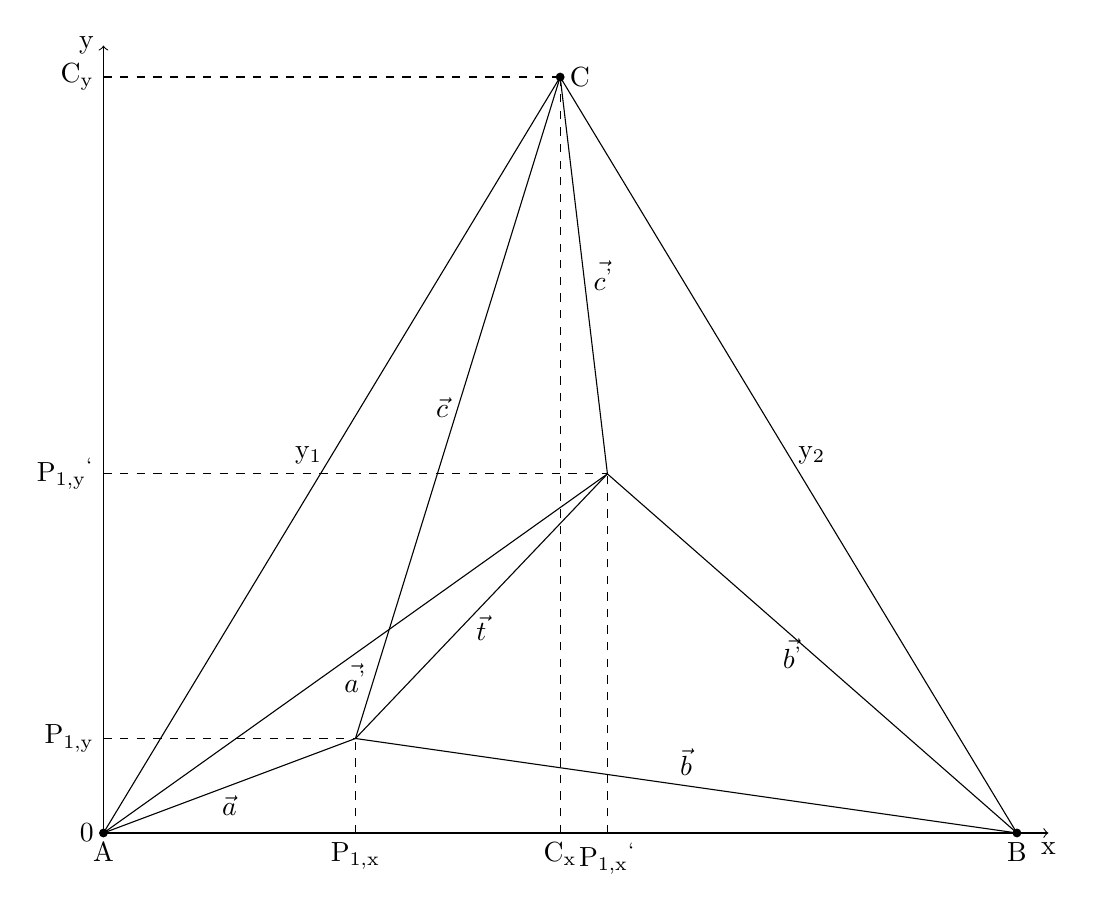
\begin{tikzpicture}[scale=0.8]
\coordinate 	[label=left:0]										(Nullpunkt) at (0,0);
\coordinate		[label=below:A] 									(A) 		at (0,0);
\coordinate		[label=below:B] 									(B) 		at (14.5,0);
\coordinate		[label=right:C] 									(C) 		at (7.25,12);

\coordinate	(P1) 		at (4,1.5) ;
\coordinate	(P1') 		at (8,5.7);

\coordinate		[label=below:x]										(X) 		at (15,0);
\coordinate		[label=left:y]										(Y) 		at (0,12.5);

\coordinate		[label=left:C\textsubscript{y}]						(YC)		at (0,12);
\coordinate		[label=below:C\textsubscript{x}]					(XC)		at (7.25,0);

\coordinate		[label=left: P\textsubscript{1,y}]					(YP1)		at (0,1.5);
\coordinate		[label=below:P\textsubscript{1,x}]					(XP1)		at (4,0);
\coordinate		[label=left: P\textsubscript{1,y}\textsuperscript{`}](YP1')		at (0,5.7);
\coordinate		[label=below:P\textsubscript{1,x}\textsuperscript{`}](XP1')		at (8,0);

\draw [->]		(Nullpunkt) -- (X)		;
\draw [->]		(Nullpunkt) -- (Y)		;
\draw 			(A) 		-- (B)		;
\draw 			(B) 		-- (C) 		node[midway,right] 	{y\textsubscript{2}};
\draw 			(C) 		-- (A) 		node[midway,left] 	{y\textsubscript{1}};
\draw 			(A) 		-- (P1) 	node[midway,below] 	{$\vec{a}$};
\draw 			(A) 		-- (P1')	node[midway,below] 	{$\vec{a\textsuperscript{'}}$};
\draw 			(B) 		-- (P1) 	node[midway,above] 	{$\vec{b}$};
\draw 			(B) 		-- (P1')	node[midway,left] 	{$\vec{b\textsuperscript{'}}$};
\draw 			(C) 		-- (P1) 	node[midway,left]  	{$\vec{c}$};
\draw 			(C) 		-- (P1')	node[midway,right]  {$\vec{c\textsuperscript{'}}$};
\draw 			(P1) 		-- (P1')	node[midway,below]  {$\vec{t}$};

\draw [dashed]  (YC) 		-- (C)		;
\draw [dashed]  (XC) 		-- (C)		;

\draw [dashed]  (YP1) 		-- (P1)		;
\draw [dashed]  (XP1) 		-- (P1)		;
\draw [dashed]  (YP1') 		-- (P1')	;
\draw [dashed]  (XP1') 		-- (P1')	;

\fill (A) circle (2pt);
\fill (B) circle (2pt);
\fill (C) circle (2pt);
\end{tikzpicture}
\caption{Darstellung der Transformation eines Punktes im Zweidimensionalen}
				
		\end{figure}
	\pagebreak
		Die Positionen der Motoren bleiben nach der Betrachtung im Zweidimensionalen identisch, jedoch wird jeder Motorposition eine Z- Koordinate hinzugefügt, sodass sich die Eckpunkte nun im Format N=(N\textsubscript{x} N\textsubscript{y} N\textsubscript{z}) befinden. Die x- und y- Komponenten bleiben bestehen, um sämtliche Vereinfachungen aus dem Zweidimensionalen übernehmen zu können.
		\begin{figure}[H]
			\centering	
			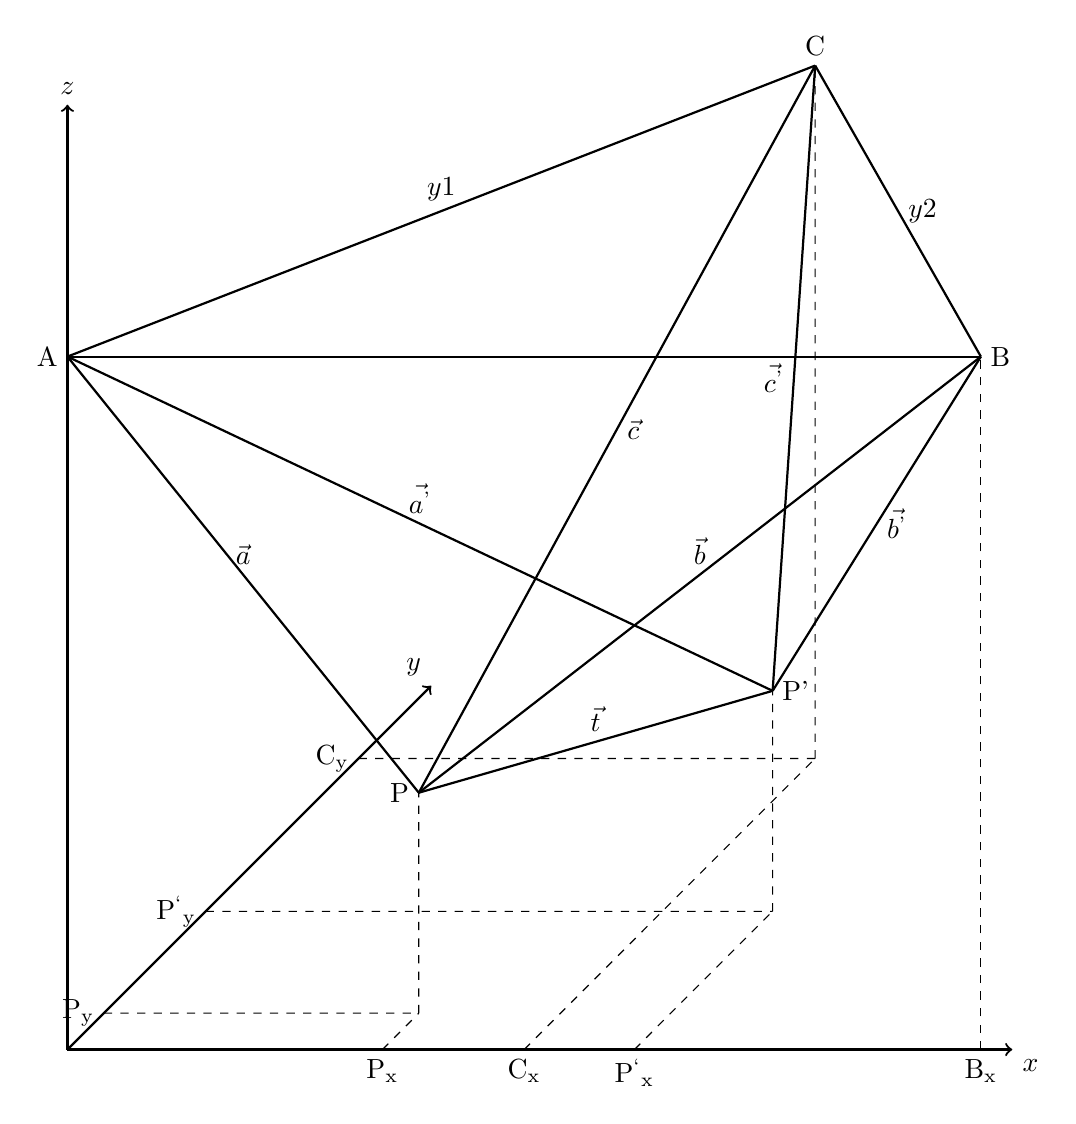
\begin{tikzpicture}[scale=0.8]
\coordinate 	[label=left:A] 										(A) 	at 	(0,11,0);
\coordinate 	[label=right:B] 									(B) 	at 	(14.5,11,0);
\coordinate 	[label=above:C] 									(C) 	at 	(7.25,11,-12);
\coordinate 	[label=left:P] 										(P) 	at 	(5,3.5,-1.5);
\coordinate 	[label=right:P'] 									(P') 	at 	(9,3.5,-5.7);

\coordinate		[label=left:P\textsubscript{y}]						(YP)	at 	(0,0,-1.5);
\coordinate		[label=below:P\textsubscript{x}]					(XP)	at 	(5,0,0);
\coordinate		[label=left:P\textsuperscript{`}\textsubscript{y}]	(YP')	at 	(0,0,-5.7);
\coordinate		[label=below:P\textsuperscript{`}\textsubscript{x}]	(XP')	at 	(9,0,0);
\coordinate		[label=below:B\textsubscript{x}]					(XB)	at 	(14.5,0,0);
\coordinate		[label=below:C\textsubscript{x}]					(XC)	at 	(7.25,0,0);
\coordinate		[label=left:C\textsubscript{y}]					    (YC)	at 	(0,0,-12);

%(x		,z		,y)
\draw[thick,->] (0,0,0) 		-- 	(15,0,0) 		node[anchor=north west]	{$x$};
\draw[thick,->] (0,0,0) 		-- 	(0,0,-15) 		node[anchor=south east]	{$y$};
\draw[thick,->] (0,0,0) 		-- 	(0,15,0) 		node[anchor=south]		{$z$};	
\draw[thick] 	(A) 			-- 	(B) 			;		
\draw[thick] 	(B) 			-- 	(C) 			node[midway,right]{$y2$};	
\draw[thick] 	(C) 			-- 	(A) 			node[midway,above]{$y1$};	
\draw[thick] 	(A) 			-- 	(P) 			node[midway,above]{$\vec{a}$};
\draw[thick] 	(A) 			-- 	(P') 			node[midway,above]{$\vec{a\textsuperscript{'}}$};
\draw[thick] 	(B) 			-- 	(P) 			node[midway,above]{$\vec{b}$};
\draw[thick] 	(B) 			-- 	(P') 			node[midway,right]{$\vec{b\textsuperscript{'}}$};
\draw[thick] 	(C) 			-- 	(P) 			node[midway,right]{$\vec{c}$};
\draw[thick] 	(C) 			-- 	(P') 			node[midway,left] {$\vec{c\textsuperscript{'}}$};
\draw[thick] 	(P) 			-- 	(P') 			node[midway,above]{$\vec{t}$};
\draw[dashed,-]  (XB) 			-- 	(B) 		;
\draw[dashed,-]  (XC) 			-- 	(7.25,0,-12) 		;
\draw[dashed,-]  (YC) 			-- 	(7.25,0,-12) 		;
\draw[dashed,-]  (7.25,0,-12) 	-- 	(C) 		;
\draw[dashed,-]  (XP) 			-- 	(5,0,-1.5) 		;
\draw[dashed,-]  (YP) 			-- 	(5,0,-1.5) 		;
\draw[dashed,-]  (5,0,-1.5) 	-- 	(P);
\draw[dashed,-]  (XP') 			-- 	(9,0,-5.7) 		;
\draw[dashed,-]  (YP') 			-- 	(9,0,-5.7) 		;
\draw[dashed,-]  (9,0,-5.7) 	-- 	(P');
\end{tikzpicture}
\caption{Darstellung der Transformation eines Punktes im Zweidimensionalen}
				
		\end{figure} 
	\pagebreak	
		Im Folgenden wird die Anpassung sämtlicher Herleitungen auf die Transformation einer Plattform erfolgen. Da zuvor die Geometrie der Eckpunkte als gleichseitiges Dreieck festgelegt wurde, wird die Plattform zu diesem Zeitpunkt ebenfalls als gleichseitiges Dreieck betrachtet, da dies den einfachsten Anwendungsfall darstellt. Sämtliche Herleitungen sind allgemein gehalten, sodass der reale Anwendungsfall für eine optimale Umsetzung der Transformation keine Anpassungen erfahren muss.	
		Die Positionen der Motoren bleiben nach der Betrachtung im Zweidimensionalen identisch, jedoch wird jeder Motorposition eine Z- Koordinate hinzugefügt, sodass sich die Eckpunkte nun im Format N=(N\textsubscript{x} N\textsubscript{y} N\textsubscript{z}) befinden. Die x- und y- Komponenten bleiben bestehen, um sämtliche Vereinfachungen aus dem Zweidimensionalen übernehmen zu können.
		\begin{figure}[H]
			\centering	
			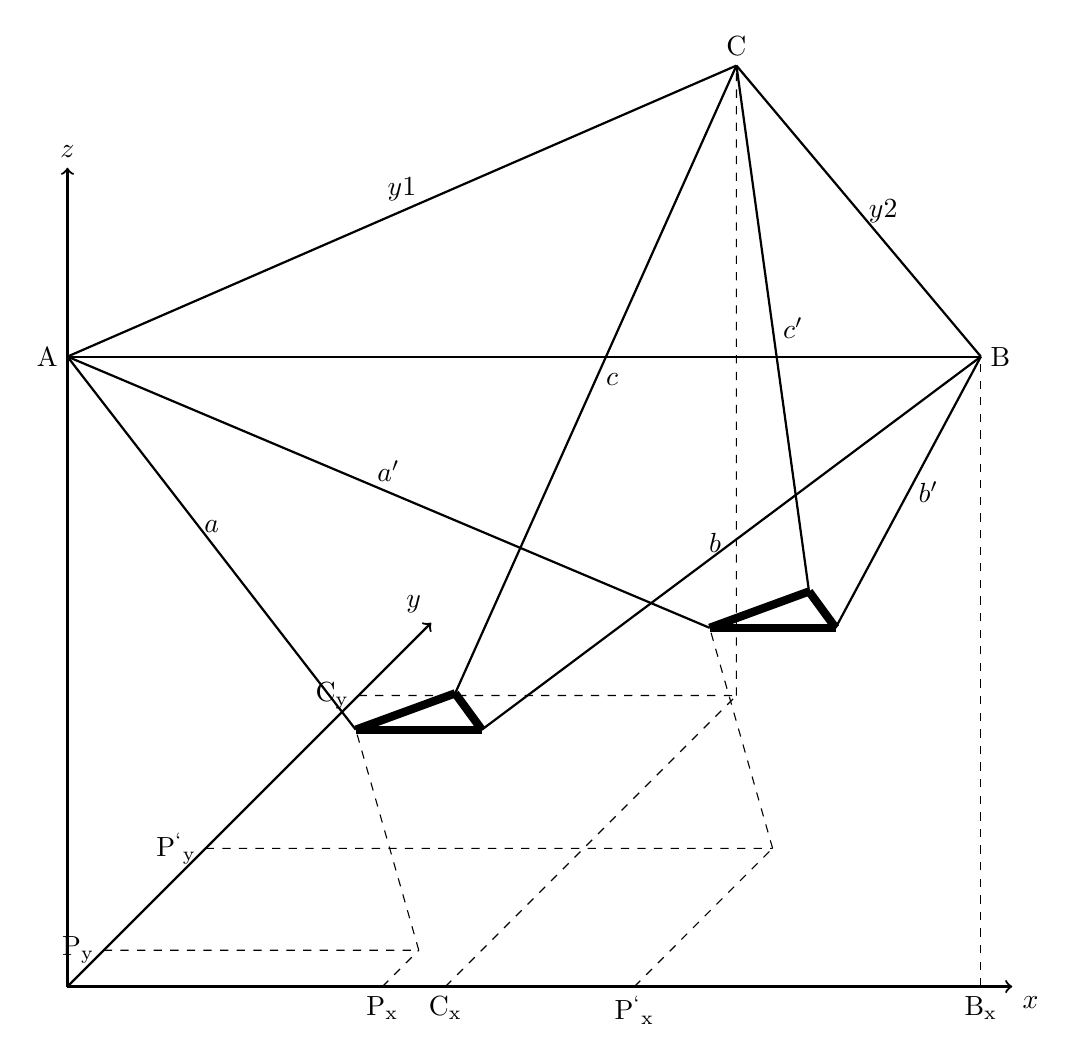
\begin{tikzpicture}[scale=0.8]		   
	\coordinate 	[label=left:	A](A) 	at 	(0,10,0);
	\coordinate 	[label=right:	B](B) 	at 	(14.5,10,0);
	\coordinate 	[label=above:	C](C) 	at 	(6,10,-12);
	\coordinate(P1) 	at 	(4,3.5,-1.5);
	\coordinate(P1') 	at 	(8,3.5,-5.7);
	\coordinate(P2) 	at 	(6,3.5,-1.5);
	\coordinate(P2') 	at 	(10,3.5,-5.7);
	\coordinate(P3) 	at 	(5,3.5,-3);
	\coordinate(P3') 	at 	(9,3.5,-7.2);
	\coordinate		[label=left:	P\textsubscript{y}](YP)	at 	(0,0,-1.5);
	\coordinate		[label=below:	P\textsubscript{x}](XP)	at 	(5,0,0);
	\coordinate		[label=left:	P\textsuperscript{`}\textsubscript{y}](YP')	at 	(0,0,-5.7);
	\coordinate		[label=below:	P\textsuperscript{`}\textsubscript{x}](XP')	at 	(9,0,0);
	\coordinate		[label=below:	B\textsubscript{x}]				(XB)	at 	(14.5,0,0);
	\coordinate		[label=below:	C\textsubscript{x}](XC)	at 	(6,0,0);
	\coordinate		[label=left:	C\textsubscript{y}](YC)	at 	(0,0,-12);

	\draw[thick,->] (0,0,0) 		-- 	(15,0,0) 	node[anchor=north west]	{$x$};
	\draw[thick,->] (0,0,0) 		-- 	(0,0,-15)	node[anchor=south east]	{$y$};
	\draw[thick,->] (0,0,0) 		-- 	(0,13,0) 	node[anchor=south]		{$z$};	
	\draw[thick] 	(A) 			-- 	(B) 		;		
	\draw[thick] 	(B) 			-- 	(C) 		node[midway,right]		{$y2$};	
	\draw[thick] 	(C) 			-- 	(A) 		node[midway,above]		{$y1$};	
	\draw[thick] 	(A) 			-- 	(P1) 		node[midway,above]		{$a$};
	\draw[thick] 	(A) 			-- 	(P1') 		node[midway,above]		{$a'$};
	\draw[thick] 	(B) 			-- 	(P2) 		node[midway,left]		{$b$};
	\draw[thick] 	(B) 			-- 	(P2') 		node[midway,right]		{$b'$};
	\draw[thick] 	(C) 			-- 	(P3) 		node[midway,right]		{$c$};
	\draw[thick] 	(C) 			-- 	(P3') 		node[midway,right]		{$c'$};
	\draw[line width =3pt] 	(P1) 			-- 	(P2) 		;
	\draw[line width =3pt] 	(P2) 			-- 	(P3) 		;
	\draw[line width =3pt] 	(P3) 			-- 	(P1) 		;
	\draw[line width =3pt] 	(P1') 			-- 	(P2') 		;
	\draw[line width =3pt] 	(P2') 			-- 	(P3') 		;
	\draw[line width =3pt] 	(P3') 			-- 	(P1') 		;
	\draw[dashed,-] (XB) 			-- 	(B) 		;
	\draw[dashed,-] (XC) 			-- 	(6,0,-12);
	\draw[dashed,-] (YC) 			-- 	(6,0,-12);
	\draw[dashed,-] (6,0,-12)	-- 	(C) 		;
	\draw[dashed,-] (XP) 			-- 	(5,0,-1.5) 	;
	\draw[dashed,-] (YP) 			-- 	(5,0,-1.5) 	;
	\draw[dashed,-] (5,0,-1.5) 		-- 	(P1)		;
	\draw[dashed,-] (XP') 			-- 	(9,0,-5.7) 	;
	\draw[dashed,-] (YP') 			-- 	(9,0,-5.7) 	;
	\draw[dashed,-] (9,0,-5.7) 		-- 	(P1')		;
\end{tikzpicture}
\caption{Darstellung der Transformation einer Plattform im Dreidimensionalen} 
		\end{figure}
	\pagebreak